\ylDisplay{Kondensaatoriredel} % Ülesande nimi
{Siim Ainsaar} % Autor
{piirkonnavoor} % Voor
{2007} % Aasta
{G 8} % Ülesande nr.
{5} % Raskustase
{
% Teema: Elektriahelad
\ifStatement
Ühesugustest kondensaatoritest mahtuvusega $C$ on koostatud joonisel näidatud lõpmatu ahel. Leidke ahela kogumahtuvus $C_k$.

\begin{center}
	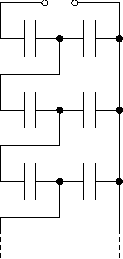
\includegraphics[width=0.3\linewidth]{2007-v2g-08-yl}
\end{center}
\fi


\ifHint
Lõpmatust ahelast ühe lüli eemaldamisega summaarne mahtuvus ei muutu.
\fi


\ifSolution
Lõpmatust ahelast ühe lüli eemaldamisega mahtuvus ei muutu. Seetõttu võime tervet ahelat vaadelda kui jadaühendust $C$-st ning $C$ ja $C_k$ paralleelühendusest. Seega saame, kasutades veel asjaolu, et jadaühenduses liituvad mahtuvuse pöördväärtused ning rööpühenduses mahtuvused ise, võrrandi:
\[
C_{k}=\frac{1}{1 / C+1 /\left(C+C_{k}\right)}.
\]
Teisendades, jõuame ruutvõrrandini:
\[
C_{k}^{2}+C C_{k}-C^{2}=0.
\]
Seda lahendades, saame:
\[
C_{k}=\frac{-1 \pm \sqrt{5}}{2} C \approx \SI{0,6}{C}.
\]
Negatiivse lahendi heitsime kõrvale.
\fi
}